% Beginning code for all standard physics latex documents

%Created on: May 8, 2014    Edited by: Wesley Kyle
%Edited on:	May 12, 2016	Edited by: P. Gimby - cleaned up the code to remove unneeded packages
%Edited on:	May 13, 2016	Edited by: P. Gimby - collected a few more packages used in 325.
%Edited on:	May 16, 2016	Edited by: P. Gimby - fixed page numbering error.
%Edited on: May 20, 2016	Edited by: Alex Shook - Added packages for 497

\documentclass[justified]{tufte-book}
\usepackage{graphicx} % allow embedded images
\setkeys{Gin}{width=\linewidth,totalheight=\textheight,keepaspectratio}
\usepackage{amsmath}  % extended mathematics
\usepackage{bm}  % bold font in math mode
\usepackage{longtable} %lets long tables flow into multiple pages instead of running off the page or having to break tables up manually
\usepackage{booktabs} % book-quality tables
\usepackage{units}    % non-stacked fractions and better unit spacing
\usepackage{multicol} % multiple column layout facilities
\usepackage{tikz} %for drawing nice pictures
\usepackage{indentfirst} % makes first line of each new section be indented
\usepackage{enumitem} % extended options for the enumerate environment
\usepackage{soul} % gives more typestting options like spacing, underline, and strike-through
\usepackage{marvosym} %extra symbols package
\usepackage{multirow} % for special table controls
\usepackage[singlelinecheck=false]{caption} % allow captions w/o figure number
\captionsetup{compatibility=false} % corrects in issue with the caption package
\usepackage{float} % allows for contorl over position of figures and tables
\allowdisplaybreaks % allows equations to span two pages if needed
\usepackage{mathrsfs} % fancy math symbols
\usepackage{multirow} % for special table controls
\usetikzlibrary{arrows,shapes,snakes,calc,patterns,3d} % addon to tikz
\usetikzlibrary{circuits.ee.IEC} % addon to tikz
\usepackage{pgfplots} % package for making plots of functions
\usepackage{gensymb} % symbols i,e. degrees
\usetikzlibrary{decorations.pathmorphing} % to draw the springs
\tikzset{circuit declare symbol = ac source}
\tikzset{set ac source graphic = ac source IEC graphic}
\usepackage{changepage} % allows for full page environment
\usepackage{comment} % allows comment tags for large sections

% define new page style that puts page numbers in the middle
%\begin{comment}
\fancypagestyle{custom}{
\fancyhf{} % clear all header and footer fields
\fancyheadoffset{0pt}
\fancyfootoffset{0pt}
\fancyfoot[C]{\thepage}
\renewcommand{\headrulewidth}{0pt}
\renewcommand{\footrulewidth}{0pt}}
\pagestyle{custom}
%\end{comment}

%below creates a new circuit symbol for AC sources
\tikzset{
         ac source IEC graphic/.style=
          {
           transform shape,
           circuit symbol lines,
           circuit symbol size = width 3 height 3,
           shape=generic circle IEC,
           /pgf/generic circle IEC/before background=
            {
             \pgftransformresetnontranslations
             \pgfpathmoveto{\pgfpoint{-0.8\tikzcircuitssizeunit}{0\tikzcircuitssizeunit}}
             \pgfpathsine{\pgfpoint{0.4\tikzcircuitssizeunit}{0.4\tikzcircuitssizeunit}}
             \pgfpathcosine{\pgfpoint{0.4\tikzcircuitssizeunit}{-0.4\tikzcircuitssizeunit}}
             \pgfpathsine{\pgfpoint{0.4\tikzcircuitssizeunit}{-0.4\tikzcircuitssizeunit}}
             \pgfpathcosine{\pgfpoint{0.4\tikzcircuitssizeunit}{0.4\tikzcircuitssizeunit}}
             \pgfusepathqstroke
            }
          }
        }
% end of circuit symbol
%\begin{document}
%%%end individual beginning code/,$d


%  \begin{titlepage}
%    \vspace*{\fill}
%    \begin{center}
%      \huge{{\bf TITLE1}}\\[0.4cm]
%      \huge{TITLE2}\\[0.4cm]
%      \LARGE{Laboratory Manual}\\[0.4cm]
%      \large{SEASON YEAR}
%    \end{center}
%    \vspace*{\fill}
%  \end{titlepage}
%\maketitle

%\begin{spacing}{0.5}
%\tableofcontents
%\end{spacing}

%NEW PHYS 497 PACKAGES AND COMMANDS

%Subcaption package: Allows subfigures to be placed side by side, and labeled with individual captions (Added June 1, 2016)
\usepackage{subcaption}

%Array package: Allows for addiation specifications in arrays (Added May 6, 2016)
\usepackage{array}

%newcolumntype: Allows one to specify a fixed column width (Added May 6, 2016)
\newcolumntype{L}[1]{>{\raggedright\let\newline\\\arraybackslash\hspace{0pt}}m{#1}}
\newcolumntype{C}[1]{>{\centering\let\newline\\\arraybackslash\hspace{0pt}}m{#1}}
\newcolumntype{R}[1]{>{\raggedleft\let\newline\\\arraybackslash\hspace{0pt}}m{#1}}

%circuits.logic.US, circuits.logic.IEC: For drawing logic gates in Tikz (Added May 6, 2016) 
\usetikzlibrary{circuits.logic.US,circuits.logic.IEC}

\newcommand{\PGT}{ %PGT: positive going transition
\begin{tikzpicture}
\draw[-angle 60] (0,0) -- (0,5pt);
\draw (0,5pt) -- (0,6pt) -- (5pt,6pt);
\draw (-5pt,0) -- (0,0);
\end{tikzpicture}
}





%TEST
\usepackage{geometry}
\pagestyle{fancy}

%\usepackage[caption=false]{subfig}

%\makeatletter
%\renewenvironment{figure}[1][htbp]{%
%  \@tufte@orig@float{figure}[#1]%
%}{%
%  \@tufte@orig@endfloat
%}

%\renewenvironment{table}[1][htbp]{%
%  \@tufte@orig@float{table}[#1]%
%}{%
%  \@tufte@orig@endfloat
%}
%\makeatother

% use instead of subfigure
\makeatletter
\newenvironment{multifigure}[1][htbp]{%
  \@tufte@orig@float{figure}[#1]%
}{%
  \@tufte@orig@endfloat
}
\makeatother

\makeatletter
\newenvironment{mainfigure}[1][htbp]{%
\@tufte@orig@float{figure}[#1]
\begin{adjustwidth}{}{-153pt}}
{\end{adjustwidth}\@tufte@orig@endfloat}%
\makeatother

\makeatletter
\newenvironment{maintable}[1][htbp]{%
\@tufte@orig@float{table}[#1]
\begin{adjustwidth}{}{-153pt}}
{\end{adjustwidth}\@tufte@orig@endfloat}%
\makeatother

%%%% Labatorial Cross-over labs need this code. This should be temporary PG Dec 7, 2016

\newcounter{questioncounter}
\setcounter{questioncounter}{0}
\newcounter{checkpointcounter}
\setcounter{checkpointcounter}{0}
\newcounter{figurecounter}
\setcounter{figurecounter}{0}
%%%%%%%%%%%%%%%%%%%%%%%%%%%%%%%%%%%%%%%%%%%%%%%%%%%%%%%

\newcommand{\checkpoint}{
 \fbox{\begin{minipage}{0.2\textwidth}
 %\includegraphics[width=0.5\textwidth]{stop}
 \end{minipage}
 \begin{minipage}{1.0\textwidth}
 {\bf CHECKPOINT \addtocounter{checkpointcounter}{1} \arabic{checkpointcounter}: Before moving on to the next part, have your TA check the results you obtained so far.}
 \end{minipage}}}

%%% end labatorial cross-over code.

% New environment for placing figure captions under the figure
%\makeatletter
%\newenvironment{mainfigure}{\textwidth}[1][htbp]{%
%\@tufte@orig@float{figure}[#1]%
%}{%
%\@tufte@orig@endfloat
%}
%\makeatother

\begin{document}
%%%%%%%%%%%%%%%%%%%%%%%%%%%%%%%%%%%%%%%%%%%%%
%
% 0079 PHYS397FA2017
%
%%%%%%%%%%%%%%%%%%%%%%%%%%%%%%%%%%%%%%%%%%%%%


\setcounter{chapter}{9}
\setcounter{equation}{0}
\setcounter{table}{0}
\setcounter{figure}{0}
\chapter{X-Ray Diffraction}

\section{Equipment}

% first column
\begin{minipage}[t]{0.5\textwidth}
\begin{itemize}[noitemsep]
\item Tel-X-ometer x-ray spectrometer
\item LiF crystal diffraction grating
\item Geiger counter detector
\item 1mm and 3mm lead collimator slides
\end{itemize}
\end{minipage}
%second column
\begin{minipage}[t]{0.5\textwidth}
\begin{itemize}[noitemsep]
\item Tel-Atomic Digicounter digital pulse counter
\item X-ray tube current monitoring cable
\item Fluke multimeter
\item Acrylic plastic x-ray attenuator slide plate
\end{itemize}
\end{minipage}

\begin{marginfigure}[+1.5in]
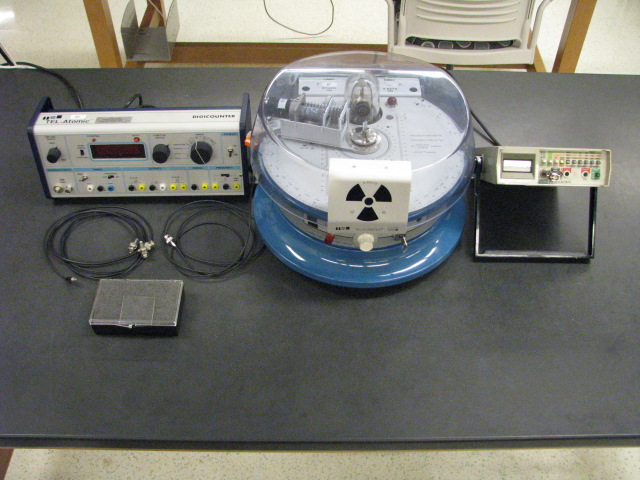
\includegraphics{/usr/local/master/labs/physics397-FA2017/0079-PHYS397FA2017/X-Ray-Diffraction-Setup.jpg}
\caption{A photograph of the experimental setup.}
\label{fig:XRsetup}
\end{marginfigure}

\section{Preparation}
Review the place of x-rays in the electromagnetic spectrum. Understand how a diffraction grating works in an optical spectrometer. Know the Planck energy relation for a quantum of light.

\section{Goals of Experiment}
\begin{itemize}
\item Introduction to x-ray crystallography.
    \item To understand how x-rays are produced and to examine the hypothesis that they are electromagnetic radiation.
    \item To understand the source of k-shell x-rays.
    \item To get experience with the control and measurement of x-rays and to work with a spectrometer that operates in the x-ray region of the electromagnetic spectrum.
\end{itemize}
%To understand how x-rays are produced and to examine the hypothesis that they are electromagnetic radiation. To be introduced to x-ray crystallography. To understand the source of k-shell x-rays. To get experience with the control and measurement of x-rays and to work with a spectrometer that operates in the x-ray region of the electromagnetic spectrum.

\section{Theory}
In the late 19th century physicists and inventors began to work with a new device called a {\bf cathode ray tube}. A cathode ray tube is a glass bulb with the air removed, a hot metal filament at one side, a metallic plate at the other end, and a high voltage between the plate and the filament. This device simultaneously started the eras of modern quantum physics and modern electronics. Among its many other properties, it was noticed that operating such a cathode ray tube at high voltages had a side effect. The cathode ray tube caused various objects outside of the tube to glow. Although other observers had noticed this effect, it was the german physicist Wilhelm R\"{o}ntgen (1845-1923) who thought it might be important and undertook a systematic study of the phenomenon.

\begin{marginfigure}
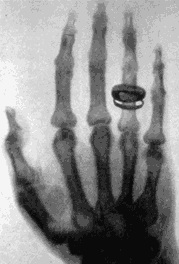
\includegraphics[width=\textwidth]{/usr/local/master/labs/physics397-FA2017/0079-PHYS397FA2017/X-Ray-Diffraction-handxray.png}
\caption{An x-ray image of a hand.}
\label{fig:xr1}
\end{marginfigure}

R\"{o}ntgen noticed that the glow persisted even when the cathode ray tube was covered up. He called the unknown emissions originating from the cathode ray tube {\bf x-rays}. A name which remains to this day, although they are also known as R\"{o}ntgen rays in his honor. Moreover, placing a hand between the glow and the tube cast an eerie shadow that illuminated the bones inside his hand in a different light than the surrounding tissue. R\"{o}ntgen found that this shadow could be photographed. Figure \ref{fig:xr1} shows one of R\"{o}ntgen's pictures, one of the earliest x-ray photographs ever taken, dating from 1895. He also found that the x-rays originated in the cathode ray tube at the location where the internal cathode rays struck the metallic plate at the end of the tube. He then established that their degree of penetration through an element depended upon its atomic number. Elements of high atomic number were able to block the x-rays better. Knowing this, he was then able to use slits cut in lead to show that x-rays travel in straight lines and that they are unaffected by electric and magnetic fields. This suggested that the x-rays were a form of electromagnetic radiation similar to light. For his work on x-rays, R\"{o}ntgen was given the 1901 Nobel prize in physics, the first ever awarded.

If x-rays were similar to light, it seemed reasonable to check whether they exhibit other optical properties of light such as {\bf diffraction}. Diffraction is a wave property of light that makes the edges cast by shadows indistinct instead of sharp and can be used to separate light of different wavelengths. Subsequent investigators had difficulty observing any diffraction and began to suspect that if x-rays were electromagnetic waves like light, they must be of a greatly different wavelength. The German physicist Max von Laue (1879-1960) realized that the spacing of atoms in crystals might be suitable for observing the diffraction of x-rays. His insight was successful and he and his students were the first people to observe {\bf x-ray diffraction} through a crystal. For this work von Laue was awarded the 1914 Nobel prize in physics.

Several more Nobel prizes were earned by physicists studying x-rays. The British son and father team of Sir William L. Bragg (1890-1971) and Sir William H. Bragg (1862-1942) extended von Laue's work. They predicted how x-rays reflect off crystals (a rule now called {\bf Bragg's law} of x-ray diffraction) and used this to design and construct instruments that can examine x-rays by their wavelength. Such instruments are now called {\bf Bragg x-ray spectrometers}. For their work the Bragg's received the 1915 Nobel prize in physics. Further work by the British physicist Charles Barkla (1877-1944) established how x-rays are scattered, polarized, and absorbed. He also discovered that each element emits its own characteristic wavelengths of x-rays which he named {\bf K-shell x-rays}. For this work Barkla received the 1917 Nobel prize in physics. More results on x-ray atomic spectra and still greater refinement of x-ray spectrometers earned the Swedish physicist Karl Siegbahn (1886-1978) a Nobel prize in 1924.

\begin{marginfigure}
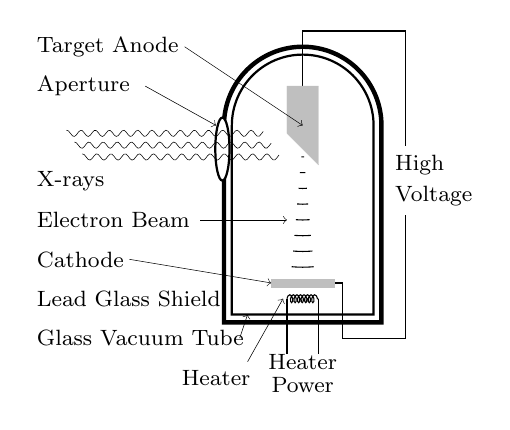
\begin{tikzpicture}
%body
\draw[ultra thick](2.5,1)--(4.5,1)--(4.5,3.5)arc(0:180:1)--cycle;
\draw[thick](2.6,1.1)--(4.4,1.1)--(4.4,3.5)arc(0:180:.9)--cycle;
\draw[thick,fill=white](2.57,3.2)arc(0:360:.9mm and 4mm);
%cathode/anode circuit
\draw[](3.5,4)--(3.5,4.7)--(4.8,4.7)--(4.8,.8)--(4,.8)--(4,1.5)--(3.5,1.5);
\draw[fill=lightgray,draw=lightgray,ultra thin](3.3,4)--(3.7,4)--(3.7,3)--(3.3,3.4)--cycle; %anode
\draw[ultra thin,draw=lightgray,fill=lightgray](3.1,1.45)rectangle(3.9,1.55); %cathode
%heater
\draw[](3.7,.6)--(3.7,1.3);
\draw[](3.3,.6)--(3.3,1.3);
\draw[decorate,decoration={coil,segment length=.45mm,amplitude=.5mm}](3.3,1.3)--(3.7,1.3); %heater coil
%electron beam
\draw[decorate,decoration={expanding waves,angle=5,segment length=2mm}](3.5,3.3)--(3.5,1.7);
%xrays
\foreach \x/\y in {0/0,.1/.15,.2/.3}{
\draw[very thin,domain=-.5:2,shift={(1+\x,3.4-\y)}] plot[samples=100] (\x,{.04*sin(\x*2000)});
}
%labels
\node[font=\footnotesize,fill=white,right]at(4.55,3){High};
\node[font=\footnotesize,fill=white,right]at(4.55,2.6){Voltage};
\node[font=\footnotesize]at(3.5,.5){Heater};
\node[font=\footnotesize]at(3.5,.2){Power};
\node[font=\footnotesize,right]at(0,4.5){Target Anode};
\draw[very thin,->](2,4.5)--(3.5,3.5);
\node[font=\footnotesize,right]at(0,4){Aperture};
\draw[very thin,->](1.5,4)--(2.4,3.5);
\node[font=\footnotesize,right]at(0,2.8){X-rays};
\node[font=\footnotesize,right]at(0,2.3){Electron Beam};
\draw[very thin,->](2.2,2.3)--(3.3,2.3);
\node[font=\footnotesize,right]at(0,1.8){Cathode};
\draw[very thin,->](1.3,1.8)--(3.1,1.5);
\node[font=\footnotesize,right]at(0,1.3){Lead Glass Shield};
\node[font=\footnotesize,right]at(0,.8){Glass Vacuum Tube};
\draw[very thin,->](2.7,.8)--(2.8,1.1);
\node[font=\footnotesize]at(2.4,.3){Heater};
\draw[very thin,->](2.8,.5)--(3.25,1.3);
\end{tikzpicture}
\caption{Schematic representation of an x-ray tube.}
\label{fig:xr2}
\end{marginfigure}

It is now accepted that x-rays are an energetic form of electromagnetic radiation with a much shorter wavelength than light. Ultimately, x-rays became a standard diagnostic tool universally used by astronomers, biologists, chemists, dentists, doctors, engineers, geologists, and physicists. The penetrating nature of x-rays makes it possible to image the interior of living organisms, observe cracks hidden in structures and mechanisms, discern the behaviour of energetic astronomical objects, study the arrangement of atoms in crystals, powders, and alloys, determine the composition of surfaces, and probe the internal energy levels of atomic isotopes.

A point most of these x-ray applications have in common is that they require an x-ray generator, a source of x-rays. Aside from refinements, the {\bf x-ray tubes} used in modern x-ray generators (and the x-ray tube used in this experiment) have the same structure as the original x-ray tubes R\"{o}ntgen used. Figure \ref{fig:xr2} shows the structure of an x-ray tube. A hot {\bf cathode} inside an evacuated glass tube emits electrons. These electrons are {\bf accelerated} to the other end of the tube by a high voltage and strike the metal target, called the {\bf anode}.  This {\bf electron beam} has enough energy to directly interact with the atoms in the target anode. Most of this energy (about 95\%) is lost in the target as heat. The remainder of the energy is converted into x-rays. The target is {\bf bevelled} to give some directionality to the emitted x-rays. Further control of the x-ray beam path is achieved by a lead glass envelope that blocks x-rays in all directions, except for the {\bf aperture} through which the x-rays are permitted to pass.

\begin{marginfigure}
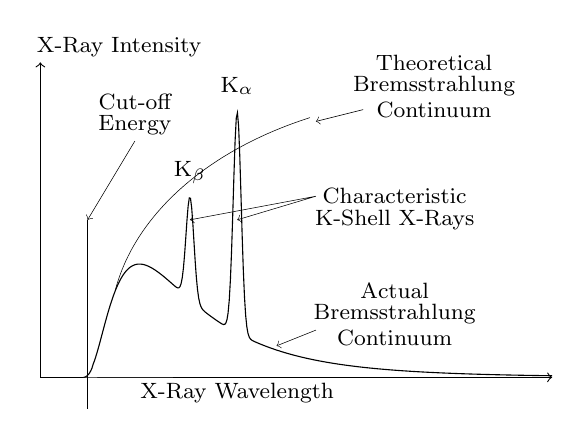
\begin{tikzpicture}
%coord system
\draw[<->](-.5,4)--(-.5,0)--(6,0);
%spectrum
\draw[domain=.05:6,fill=white] plot [samples=400] (\x, {1.3*exp(-(\x-1.4)*(\x-1.4)*200)+2.8*exp(-(\x-2)*(\x-2)*200)+1.4*exp(-1*ln(\x*.8)*ln(\x*.8))/\x});
\draw[very thin](.45,1.1)arc(170:115:4.4 and 3);
\draw[thin](0.1,-.4)--(0.1,2);
%labels
\node[font=\footnotesize]at(.7,3.5){Cut-off};
\node[font=\footnotesize]at(.7,3.2){Energy};
\draw[very thin,->](.7,3)--(.1,2);
\node[font=\footnotesize]at(.5,4.2){X-Ray Intensity};
\node[font=\footnotesize]at(2,3.7){K$_\alpha$};
\node[font=\footnotesize]at(1.4,2.6){K$_\beta$};
\node[font=\footnotesize]at(2,-.2){X-Ray Wavelength};
\node[font=\footnotesize]at(4.5,4){Theoretical};
\node[font=\footnotesize]at(4.5,3.7){Bremsstrahlung};
\node[font=\footnotesize]at(4.5,3.4){Continuum};
\draw[->,very thin](3.6,3.4)--(3,3.25);
\node[font=\footnotesize]at(4,2.3){Characteristic};
\node[font=\footnotesize]at(4,2){K-Shell X-Rays};
\draw[very thin,<->](1.4,2)--(3,2.3)--(2,2);
\node[font=\footnotesize]at(4,1.1){Actual};
\node[font=\footnotesize]at(4,.8){Bremsstrahlung};
\node[font=\footnotesize]at(4,.5){Continuum};
\draw[very thin,->](3,.6)--(2.5,.4);
\end{tikzpicture}
\caption{An example of an x-ray spectrum.}
\label{fig:xr3}
\end{marginfigure}

The x-rays generated by a typical x-ray tube cover a broad range of wavelengths. The proportion of x-rays at any given wavelength is governed by the physical interaction processes between the electrons in the electron beam and the atoms inside the target. A typical spectrum of x-rays emitted by an x-ray tube is shown in Figure \ref{fig:xr3}. It can be seen that the spectrum exhibits two main features. There is a broad curve at all wavelengths to the right of a certain value. Superimposed on this is a set of sharp peaks. It has been found the shape of the smooth part is determined by the magnitude of the high voltage and the aperture material. The positions and relative sizes of the sharp peaks is determined by the type of atoms the target anode is composed of.

The smooth broad curve is known as the {\bf bremsstrahlung continuum}. This bremsstrahlung radiation, or {\bf braking radiation}, arises due to the acceleration the electrons undergo when they strike the target anode and interact with the electric fields of the atoms inside. Electromagnetic theory predicts that accelerated charges will {\bf radiate} electromagnetic waves. The large number of electrons in the electron beam are all accelerating in different ways since they interact with different atoms of the target at a variety of distances. So the radiated electromagnetic energy happens at many wavelengths and this yields the continuum.

According to the quantum picture, this radiation will be in the form of photons with energy $E = h\nu$ corresponding to the change in the electron kinetic energy $\Delta$ K, so that

\begin{equation}
E=h\nu =\Delta K
\label{equ:xr1}
\end{equation}

\noindent where $\nu$ is the frequency of the photon, and $h = 6.62606876\times10^{-34}$ Js is {\bf Planck's constant}.

The most energetic possible photon occurs when the electron loses all of its kinetic energy in a single interaction. For an x-ray tube with accelerating voltage, V, the maximum photon energy, E$_{max}$ , and corresponding minimum wavelength $\lambda_{min}$ is

\begin{equation}
E_{max}=h\nu_{max}=\dfrac{hc}{\lambda_{min}}=eV
\label{equ:xr2}
\end{equation}

\begin{marginfigure}
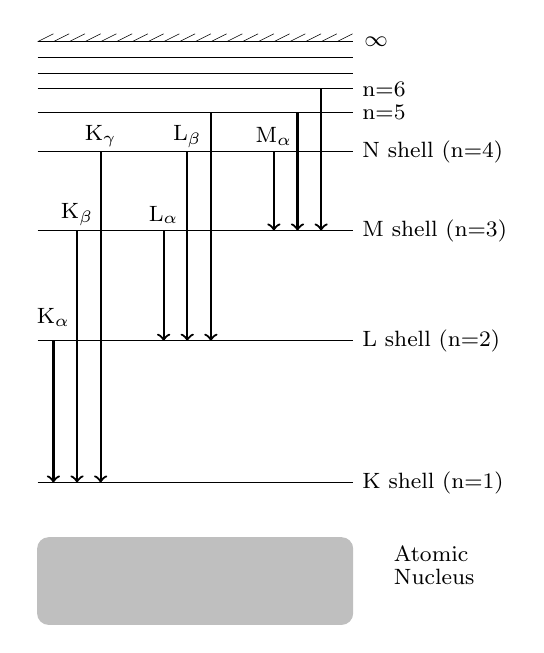
\begin{tikzpicture}
%E levels
\draw[](0,0)--(4,0);
\draw[](0,-.2)--(4,-.2);
\draw[](0,-.4)--(4,-.4);
\foreach \y in {0,1.5,4,9,16,25}{
\draw[](0,-.6-\y*.2)--(4,-.6-\y*.2);
}
%transition arrows
\draw[->,thick](.2,-3.8)--(.2,-5.6);
\draw[->,thick](.5,-2.4)--(.5,-5.6);
\draw[->,thick](.8,-1.4)--(.8,-5.6);

\draw[->,thick](1.6,-2.4)--(1.6,-3.8);
\draw[->,thick](1.9,-1.4)--(1.9,-3.8);
\draw[->,thick](2.2,-.9)--(2.2,-3.8);

\draw[->,thick](3,-1.4)--(3,-2.4);
\draw[->,thick](3.3,-.9)--(3.3,-2.4);
\draw[->,thick](3.6,-.6)--(3.6,-2.4);
%nucleus box
\draw[draw=lightgray,fill=lightgray,rounded corners=4pt](0,-7.4)rectangle(4,-6.3);
%shading at top
\foreach \x in {0,...,19}{
\draw[very thin](0+\x*.2,0)--(.2+\x*.2,.1);
}
%labels
\node[font=\footnotesize]at(.2,-3.5){K$_\alpha$};
\node[font=\footnotesize]at(.5,-2.2){K$_\beta$};
\node[font=\footnotesize]at(.8,-1.2){K$_\gamma$};
\node[font=\footnotesize]at(1.6,-2.2){L$_\alpha$};
\node[font=\footnotesize]at(1.9,-1.2){L$_\beta$};
\node[font=\footnotesize]at(3,-1.2){M$_\alpha$};
\node[font=\footnotesize]at(4.3,0){$\infty$};
\node[font=\footnotesize,right]at(4,-.6){n=6};
\node[font=\footnotesize,right]at(4,-.9){n=5};
\node[font=\footnotesize,right]at(4,-1.4){N shell (n=4)};
\node[font=\footnotesize,right]at(4,-2.4){M shell (n=3)};
\node[font=\footnotesize,right]at(4,-3.8){L shell (n=2)};
\node[font=\footnotesize,right]at(4,-5.6){K shell (n=1)};
\node[font=\footnotesize,right]at(4.4,-6.5){Atomic};
\node[font=\footnotesize,right]at(4.4,-6.8){Nucleus};
\end{tikzpicture}
\caption{Diagram representing electronic energy levels in an atom.}
\label{fig:xr4}
\end{marginfigure}

\noindent where $e = 1.60217646\times10^{-19}$ C is the charge of an electron and c = 299792458 m/s is the speed of light. This highest energy is known as the {\bf cut-off energy} of the x-ray tube. An x-ray tube cannot generate x-rays with higher energy than the cut-off energy. At the low end of the spectrum, it seems reasonable to expect that low energy x-rays would be produced in much greater quantities than high energy x-rays near the cut-off. Theoretically, this is indeed correct as can be seen by the theoretical curve shown in Figure \ref{fig:xr3}. However, in practice, it turns out that the low energy x-rays are not detected in great numbers. The reason for this is that low energy x-rays are easily absorbed. The lowest energy x-rays do not even make it out of the target material. Still more are blocked by the glass walls of the x-ray tube, the air, and the entrance walls of the x-ray detector. This results in the characteristic shape of the bremsstrahlung spectrum seen in Figure \ref{fig:xr3}, where numbers of x-rays are small at low energies, increase to some maximum, and then decrease back down to zero at the cut-off.

The other feature of the x-ray tube spectrum is seen to be the sharp peaks that rise above the bremsstrahlung continuum. These peaks are also due to interactions between the electrons in the electron beam and the atoms in the target. The energy level model of the atom implies that the electrons surrounding the nucleus of an atom have different energy levels called {\bf shells}. Each electron shell has a designated {\bf principal quantum number}, n. As seen in Figure \ref{fig:xr4}, the innermost shell has quantum number n=1 and is commonly called the {\bf K-shell}. The next shell outward has quantum number n=2 and so on. Any transition of an electron from one level to a lower level must be accompanied by the emission of a photon of energy equal to the energy difference between the two levels.

Electrons in the electron beam of the x-ray tube which are sufficiently energetic can penetrate into the atoms and knock an electron out of an inner shell. In turn, an electron from a higher energy level falls down to fill the hole in the inner shell and thereby releases a photon of the corresponding energy difference. So, for example, when an inner electron from the K-shell is removed from the atom, a common transition is for an electron in the next higher shell (n = 2) to move into the inner shell and emit a photon. As seen in Figure \ref{fig:xr4}, this photon is named K$_{\alpha}$. It turns out that for many materials, the K$_{\alpha}$ photon (and many others) happens to have sufficient energy to be an x-ray photon. Each element has a characteristic set of x-ray peaks corresponding to transitions of electrons between inner energy levels. The height of each peak is related to the probability that the particular electron transition corresponding to that energy difference can happen. These {\bf characteristic x-rays} serve as an identifying marker that can be used to identify the target material and explore its inner atomic energy levels.

\begin{marginfigure}
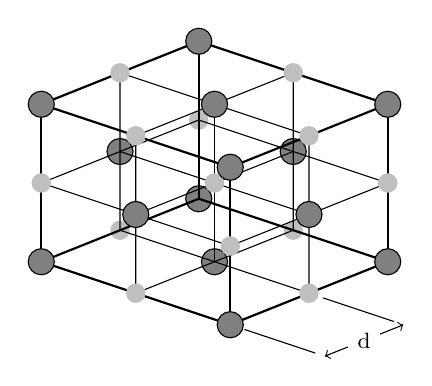
\begin{tikzpicture}[y={(-.6cm,0.2cm)},x={(.5cm,.2cm)}, z={(0cm,.5cm)}]
% coordinate system
\coordinate (O) at (0, 0, 0);
\node[circle,scale=1,fill=gray,draw]at(2,2,0){};
\node[circle,scale=1,fill=gray,draw]at(2,0,2){};
\node[circle,scale=1,fill=gray,draw]at(0,2,2){};
\node[circle,scale=1,fill=gray,draw]at(0,0,0){};
\node[circle,scale=.7,fill=lightgray,draw=lightgray]at(2,2,2){};
\node[circle,scale=.7,fill=lightgray,draw=lightgray]at(2,0,0){};
\node[circle,scale=.7,fill=lightgray,draw=lightgray]at(0,2,0){};
%bonds
\draw[thick](-2,-2,0)--(-2,2,0)--(2,2,0)--(2,-2,0)--cycle;
\draw[thick](-2,-2,4)--(-2,2,4)--(2,2,4)--(2,-2,4)--cycle;
\draw[thick](-2,-2,0)--(-2,-2,4);
\draw[thick](-2,2,0)--(-2,2,4);
\draw[thick](2,-2,0)--(2,-2,4);
\draw[thick](2,2,0)--(2,2,4);
\draw[](-2,-2,2)--(-2,2,2)--(2,2,2)--(2,-2,2)--cycle;
\draw[](0,-2,4)--(0,-2,0)--(0,2,0)--(0,2,4)--cycle;
\draw[](-2,0,0)--(-2,0,4)--(2,0,4)--(2,0,0)--cycle;
\draw[](0,-2,2)--(0,2,2);
\draw[](2,0,2)--(-2,0,2);
\draw[](0,0,4)--(0,0,0);
%atoms
\node[circle,scale=.7,fill=lightgray,draw=lightgray]at(0,0,2){};
\node[circle,scale=1,fill=gray,draw]at(-2,-2,0){};
\node[circle,scale=1,fill=gray,draw]at(2,-2,0){};
\node[circle,scale=1,fill=gray,draw]at(-2,2,0){};
\node[circle,scale=1,fill=gray,draw]at(2,2,4){};
\node[circle,scale=1,fill=gray,draw]at(2,-2,4){};
\node[circle,scale=1,fill=gray,draw]at(-2,2,4){};
\node[circle,scale=1,fill=gray,draw]at(-2,-2,4){};
\node[circle,scale=1,fill=gray,draw]at(0,-2,2){};
\node[circle,scale=1,fill=gray,draw]at(-2,0,2){};
\node[circle,scale=1,fill=gray,draw]at(0,0,4){};
\node[circle,scale=.7,fill=lightgray,draw=lightgray]at(-2,0,0){};
\node[circle,scale=.7,fill=lightgray,draw=lightgray]at(0,-2,0){};
\node[circle,scale=.7,fill=lightgray,draw=lightgray]at(-2,0,4){};
\node[circle,scale=.7,fill=lightgray,draw=lightgray]at(0,-2,4){};
\node[circle,scale=.7,fill=lightgray,draw=lightgray]at(0,2,4){};
\node[circle,scale=.7,fill=lightgray,draw=lightgray]at(2,0,4){};
\node[circle,scale=.7,fill=lightgray,draw=lightgray]at(-2,2,2){};
\node[circle,scale=.7,fill=lightgray,draw=lightgray]at(2,-2,2){};
\node[circle,scale=.7,fill=lightgray,draw=lightgray]at(-2,-2,2){};
%label
\draw[<->](0,-4,0)--(-2,-4,0);
\draw[](0,-2.3,0)--(0,-3.8,0);
\draw[](-2,-2.3,0)--(-2,-3.8,0);
\node[font=\footnotesize,fill=white]at(-1,-4,0){d};
\end{tikzpicture}
\caption{Crystalline structure of a Lithium Fluoride.}
\label{fig:xr5}
\end{marginfigure}

It is therefore of strong interest to find a method to determine the wavelengths of the features seen in the x-ray spectrum because the actual wavelengths could be used to measure the energy levels of electronic orbitals inside the atom. What is needed is a device that can separate x-rays by their wavelength. For visible light, the device commonly used for this purpose is called a {\bf diffraction grating}. It consists of a large number of equally spaced parallel lines inscribed onto glass. The spacing of the lines is critical to the operation of the grating. For useable results, the separation between the lines should be roughly the same size or smaller than the wavelength of the light to be diffracted. So for visible light with a wavelength around 500 nm, the spacing of the lines needs to be at least 200 lines per millimeter. Unfortunately, it turns out that the wavelength of x-rays is about 1000 times smaller than the wavelength of visible light. It is quite difficult to machine lines fine enough to serve as a diffraction grating for x-rays. However, the spacing between atoms in a regular solid such as a {\bf crystal} serves very well as a {\bf natural} diffraction grating for x-rays.

This natural correspondence between the x-ray wavelength and the spacing of atoms enables crystals to be used as diffraction gratings for x-rays. The study of crystals and x-rays constitutes the scientific field of {\bf x-ray crystallography}. There is a large abundance of different types of crystals, each with their own structure and properties. This experiment restricts its attention to the simplest type of crystal, an ionic solid with a {\bf cubic structure} as seen in Figure \ref{fig:xr5}. The most common example of this type of solid is ordinary table salt, NaCl. Unfortunately, salt crystals have a tendency to absorb water and break down. For this reason, the cubic ionic crystal used in this experiment instead is {\bf Lithium Fluoride, LiF}. As seen in Figure 5, each atom of lithium is surrounded by six fluorine atoms and conversely, each fluorine atom is surrounded by six lithium atoms. All of the atoms are the same distance from each other and this gives rise to the cubic crystal structure.

It seems reasonable to expect that the spacing between the atoms in the LiF crystal influences how the x-rays diffract through the crystal in the same way that the spacing between ruled lines determines how visible light diffracts through an optical diffraction grating. The cubic structure of LiF makes it possible to calculate the distance between the atoms. Let the {\bf atomic mass} of lithium be denoted by A$_{Li}$ and the atomic mass of fluorine be denoted by A$_F$. Then the {\bf molar mass}, A$_{LiF}$, of lithium fluoride is given by

\begin{equation}
A_{LiF}=A_{Li}+A_F
\label{equ:xr3}
\end{equation}

\noindent The number of molecules in A$_{LiF}$ grams of LiF is N$_A$, where N$_A=6.02214199\times10^{23}$ is {\bf Avogadro's number}. If the density of LiF is $\rho$ grams per cubic centimeter, then the volume, V, of N$_A$ molecules of LiF must be

\begin{equation}
V=\dfrac{A_{LiF}}{\rho}
\label{equ:xr4}
\end{equation}

\noindent cubic centimeters. Since LiF is {\bf diatomic}, the {\bf atomic spacing}, d, in centimeters, between the atoms in LiF is

\begin{equation}
d=\sqrt[3]{\dfrac{A_{LiF}}{2N_A\rho}}
\label{equ:xr5}
\end{equation}

\begin{marginfigure}
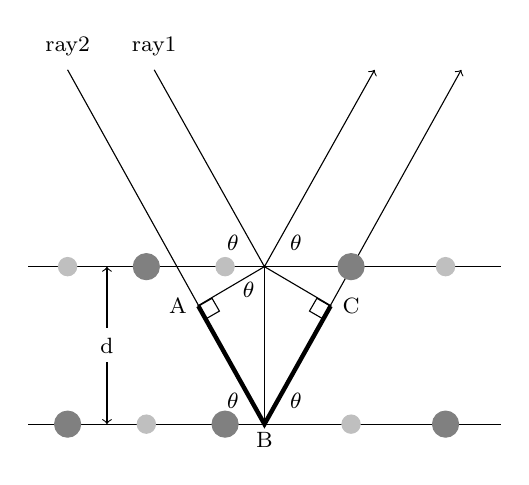
\begin{tikzpicture}
%lines and arrows
\draw[](0,0)--(6,0);
\draw[](0,2)--(6,2);
\draw[->](.5,4.5)--(3,0)--(5.5,4.5);
\draw[->](1.6,4.5)--(3,2)--(4.4,4.5);
\draw[](2.15,1.5)--(3,2)--(3.85,1.5);
\node[rectangle,draw,scale=.8,rotate=30]at(2.3,1.47){};
\node[rectangle,draw,scale=.8,rotate=60]at(3.7,1.47){};
\draw[](3,2)--(3,0);
\draw[ultra thick](2.16,1.5)--(3,0)--(3.84,1.5);
\draw[<->](1,0)--(1,2);
%atoms
\foreach \x/\y in {.5/0,1.5/2,4.1/2,5.3/0,2.5/0}{
\node[circle,draw=gray,fill=gray]at(\x,\y){};
}
\foreach \x/\y in {.5/2,1.5/0,2.5/2,4.1/0,5.3/2}{
\node[circle,draw=lightgray,fill=lightgray,scale=.7]at(\x,\y){};
}
%labels
\node[fill=white,font=\footnotesize]at(1,1){d};
\node[font=\footnotesize]at(1.6,4.8){ray1};
\node[font=\footnotesize]at(.5,4.8){ray2};
\node[font=\footnotesize]at(1.9,1.5){A};
\node[font=\footnotesize]at(3,-.2){B};
\node[font=\footnotesize]at(4.1,1.5){C};
\node[font=\footnotesize]at(2.6,.3){$\theta$};
\node[font=\footnotesize]at(3.4,.3){$\theta$};
\node[font=\footnotesize]at(2.6,2.3){$\theta$};
\node[font=\footnotesize]at(3.4,2.3){$\theta$};
\node[font=\footnotesize]at(2.8,1.7){$\theta$};
\end{tikzpicture}
\caption{A geometrical perspective on x-ray interaction with a LiF substrate.}
\label{fig:xr6}
\end{marginfigure}

To calculate how the diffraction of x-rays happens inside an LiF crystal, assume that the LiF has a cubic structure and that the x-rays actually are electromagnetic waves. The separation, d, between  two neighboring atomic planes is then given by Equation \ref{equ:xr5}. Imagine two x-rays, ray1 and ray2, with wavelength, $\lambda$, reflecting off of two planes of atoms inside the crystal with angle of incidence $\theta$ as seen in Figure \ref{fig:xr6}. For electromagnetic waves, the angle of reflection equals the angle of incidence, so the reflected ray also leaves the crystal at the same angle $\theta$. If ray1 and ray2 are parallel, then the extra distance travelled by ray2 is the length of the two line segments AB and BC. For {\bf constructive interference} to occur, the distance AB+BC must be an integer multiple of the wavelength. So when x-rays reflect off of the surface of a LiF crystal, each wavelength reflects at a particular angle and all the other wavelengths cancel out. The length of AB is $d\cdot sin(\theta)$, so the condition for constructive interference is

\begin{equation}
n\lambda=2d\sin(\theta)\hspace{4mm} n=1,2,...
\label{equ:xr6}
\end{equation}

This formula is known as {\bf Braggs law} and it describes how x-rays diffract when reflected by a cubic crystal. This diffraction interaction is called {\bf Bragg x-ray diffraction} and it implies that a LiF crystal can be used to measure the wavelength of x-rays simply by tilting it at different angles to the x-ray beam.

The instrument that measures an x-ray spectrum by taking advantage of Bragg's law is called a {\bf Bragg x-ray spectrometer}. The construction of a typical Bragg x-ray spectrometer is shown in Figure \ref{fig:xr7}. An x-ray tube generates a beam of x-rays. The x-ray tube is operated by an

\begin{figure}
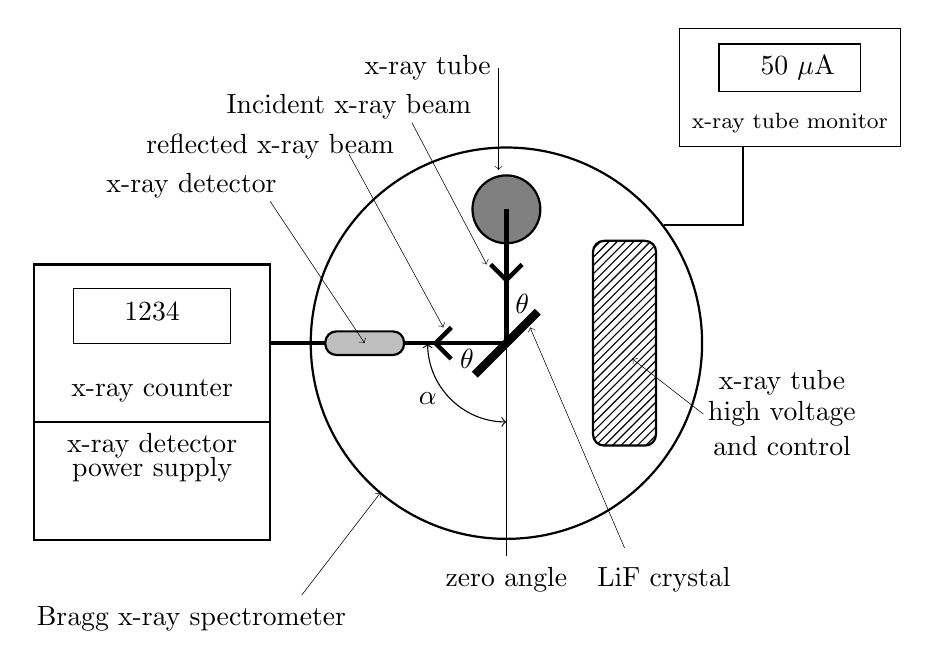
\begin{tikzpicture}
%tube monitor
\draw[](8.2,6.5)rectangle(11,8);
\draw[](8.7,7.2)rectangle(10.5,7.8);
\draw[thick](9,6.5)--(9,5.5)--(8,5.5);
\node[circle,scale=15,draw,thick]at(6,4){}; %base
%counter and power supply
\draw[thick](0,1.5)rectangle(3,5);
\draw[](.5,4)rectangle(2.5,4.7);
\draw[thick](0,3)--(3,3);
\node[circle,draw,rounded corners=4pt,thick,fill=gray,scale=2.6]at(6,5.7){};
\draw[ultra thick](3,4)--(6,4)--(6,5.7); %xray path
\draw[line width=3pt](5.6,3.6)--(6.4,4.4);
%xray detector
\node[rectangle,draw,rounded corners=4pt,thick,fill=lightgray,minimum width=1cm,minimum height=3mm]at(4.2,4){};
\draw{}(6,4)--(6,1.3);
%high voltage and control
\node[rectangle,draw,rounded corners=4pt,thick,pattern=north east lines,minimum width=.8cm,minimum height=2.6cm]at(7.5,4){};
%angle line and x-ray beam arrows
\draw[thin,<->](6,3)arc(-90:-180:1);
\draw[ultra thick](5.8,5)--(6,4.8)--(6.2,5);
\draw[ultra thick](5.3,4.2)--(5.1,4)--(5.3,3.8);
%labels
\node[]at(5,3.3){$\alpha$};
\node[]at(5.5,3.8){$\theta$};
\node[]at(6.2,4.5){$\theta$};
\node[]at(9.7,7.5){50 $\mu$A};
\node[]at(1.5,4.4){1234};
\node[]at(1.5,3.4){x-ray counter};
\node[]at(1.5,2.7){x-ray detector};
\node[]at(1.5,2.4){power supply};
\node[font=\footnotesize]at(9.6,6.8){x-ray tube monitor};
\node[]at(8,1){LiF crystal};
\draw[very thin,->](7.5,1.4)--(6.3,4.2);
\node[]at(5,7.5){x-ray tube};
\draw[very thin,->](5.9,7.5)--(5.9,6.2);
\node[]at(4,7){Incident x-ray beam};
\draw[very thin,->](4.8,6.8)--(5.75,5);
\node[]at(3,6.5){reflected x-ray beam};
\draw[very thin,->](4,6.4)--(5.2,4.2);
\node[]at(2,6){x-ray detector};
\draw[very thin,->](3,5.8)--(4.2,4);
\node[]at(2,.5){Bragg x-ray spectrometer};
\draw[very thin,->](3.4,.8)--(4.4,2.1);
\node[]at(6,1){zero angle};
\node[]at(9.5,3.5){x-ray tube};
\node[]at(9.5,3.1){high voltage};
\node[]at(9.5,2.7){and control};
\draw[very thin,->](8.5,3.1)--(7.6,3.8);
\end{tikzpicture}
\caption{An example of a typical Bragg x-ray spectrometer.}
\label{fig:xr7}
\end{figure}

\noindent associated high voltage power supply together with control and monitoring electronics. The x-ray beam strikes a mounted crystal at some incident angle $\theta$. Bragg diffraction suggests that the reflected x-rays at the same angle $\theta$ will be at the single x-ray wavelength given by Bragg's law, Equation \ref{equ:xr6}. The reflected beam is detected by an {\bf x-ray detector}. An x-ray detector measures the intensity of the reflected beam. Usually this is done by counting the number of arriving x-ray photons. The x-ray detector also requires its own power supply and control system.

The apparatus is arranged so that the detector can be rotated to any angle $\alpha$. An internal mechanism links the rotation of the detector to the rotation of the crystal. This is done so that for any detector angle, $\alpha$, the crystal is positioned such that the angle of incidence, $\theta$, equals the angle of reflection, $\theta$, as seen in Figure \ref{fig:xr7}. The angle $\alpha$ is always twice the angle $\theta$ so that

\begin{equation}
\alpha=2\theta
\label{equ:xr7}
\end{equation}

\noindent In this way the number of x-rays at any wavelength is determined and when the resulting data is plotted, an x-ray spectrum such as the one in Figure \ref{fig:xr3} is obtained. The crystal spacing and Equation \ref{equ:xr6} can then be used to relate an x-ray wavelength to each angle . Equation \ref{equ:xr6} also suggests that {\bf higher order} spectral features may be visible when $n = 2, 3,...$ . In general, higher order spectra are less bright (a smaller number of x-ray photons) than the primary ($n=1$) spectrum because the extra travel distance through the crystal increases the probablity that the x-ray photon will be absorbed inside the crystal.
	A more detailed view of the Bragg spectrometer actually used in this experiment is shown in Figure \ref{fig:xr8}. The most significant addition to the instrument are {\bf safety interlocks} and {\bf shielding}. Due to their penetrating nature, x-rays are considered to be harmful radiation when received in

\begin{figure}
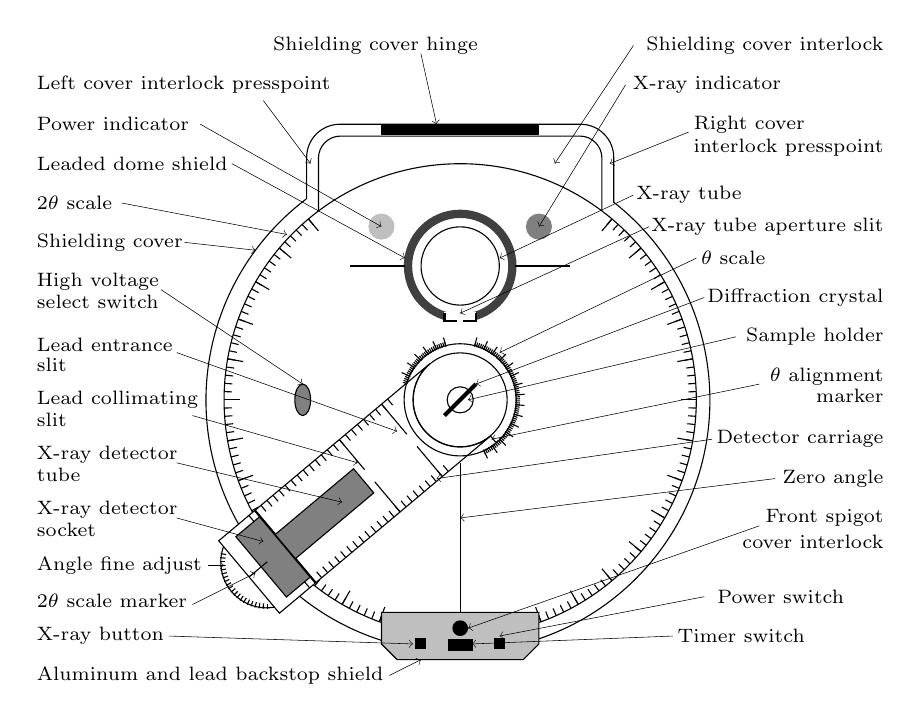
\begin{tikzpicture}
%large circle with tics
\node[circle,scale=18.1,draw]at(0,0){};
\foreach \r in {40,50,...,160}{
\draw[rotate=\r](0,2.8)--(0,3);
\draw[rotate={180-\r}](0,-2.8)--(0,-3);
}
\foreach \r in {40,42,...,160}{
\draw[rotate=\r](0,2.9)--(0,3);
\draw[rotate={180-\r}](0,-2.9)--(0,-3);
}
%shielding
\draw[](1.95,2.51)arc(51.8:-233:3.2);
\draw[rounded corners=12pt](-1.95,2.55)--(-1.95,3.5)--(1.95,3.5)--(1.95,2.5);
\draw[rounded corners=8pt](-1.8,2.4)--(-1.8,3.35)--(1.8,3.35)--(1.8,2.4);
\draw[line width=3.8pt](-1,3.43)--(1,3.43);
%detector tube assembly
\begin{scope}[rotate=-50]
\node[circle,draw,scale=3.6]at(0,0){};
\draw[fill=white](.6,0)--(.6,-3.5)--(-.6,-3.5)--(-.6,0)arc(180:360:.6);
\draw[](.5,-3.5)arc(-30:-150:.58);
\draw[fill=gray,draw=black](-.5,-3.3)rectangle(.5,-2.9);
\draw[thick](-.6,-2.9)--(.6,-2.9);
\draw[fill=gray,draw=black](-.2,-2.9)rectangle(.2,-1.6);
\draw[](-.6,-1.5)--(-.1,-1.5);
\draw[](-.6,-.8)--(-.1,-.8);
\draw[](.6,-1.5)--(.1,-1.5);
\draw[](.6,-.8)--(.1,-.8);
\foreach \y in {.1,.2,...,2.4}{
\draw[](-.6,-.6-\y)--(-.5,-.6-\y);
\draw[](.5,-.6-\y)--(.6,-.6-\y);
}
\foreach \r in {0,5,...,100}{
\draw[shift={(0cm,-3.2cm)},rotate={-40-\r}](.53,0)--(.6,0);
}
\draw[](.6,0)--(.7,0);
\draw[](0,-3.5)--(0,-3.2);
\end{scope}
%center angle scale and diffraction crystal
\node[circle,draw,scale=4.3]at(0,0){};
\foreach \r in {0,10,...,140}{
\draw[rotate={-15-\r}](0,.7)--(0,.82);
}
\foreach \r in {0,2,...,140}{
\draw[rotate={-15-\r},thin](0,.7)--(0,.76);
}
\foreach \r in {0,10,...,50}{
\draw[rotate={15+\r}](0,.7)--(0,.82);
}
\foreach \r in {0,2,...,58}{
\draw[rotate={15+\r},thin](0,.7)--(0,.76);
}
\node[circle,draw,scale=1]at(0,0){};
\draw[line width=1.5pt](-.2,-.2)--(.2,.2);
%x-ray tube
\node[circle,draw=darkgray,line width=3pt,scale=4]at(0,1.7){};
\node[circle,draw,scale=3]at(0,1.7){};
\node[rectangle,fill=white,minimum width=4mm]at(0,1){};
\draw[thick](-.2,1.1)--(-.2,1)--(-.04,1);
\draw[thick](.2,1.1)--(.2,1)--(.04,1);
\draw[](-1.4,1.7)--(-.7,1.7);
\draw[](1.4,1.7)--(.7,1.7);
%indicators and switches
\node[circle,fill=gray]at(1,2.2){};
\node[circle,fill=lightgray]at(-1,2.2){};
\draw[fill=gray](-2,0)ellipse(1mm and 2mm){};
%zero line
\draw[](0,-.8)--(0,-3);
%control panel and backstop shield
\draw[fill=lightgray](-1,-3.1)--(-1,-2.7)--(1,-2.7)--(1,-3.1)--(.8,-3.3)--(-.8,-3.3)--cycle;
\node[circle,fill,scale=.6]at(0,-2.9){};
\node[rectangle,fill,scale=.6]at(.5,-3.1){};
\node[rectangle,fill,scale=.6]at(-.5,-3.1){};
\draw[fill](-.15,-3.18)rectangle(.15,-3.05);
%labels
\node[right,font=\scriptsize]at(-2.5,4.5){Shielding cover hinge};
\draw[very thin,->](-.5,4.4)--(-.3,3.5);
\node[right,font=\scriptsize]at(-5.5,4){Left cover interlock presspoint};
\draw[very thin,->](-2.5,3.8)--(-1.9,3);
\node[right,font=\scriptsize]at(-5.5,3.5){Power indicator};
\draw[very thin,->](-3.3,3.5)--(-1,2.2);
\node[right,font=\scriptsize]at(-5.5,3){Leaded dome shield};
\draw[very thin,->](-2.9,3)--(-.7,1.8);
\node[right,font=\scriptsize]at(-5.5,2.5){2$\theta$ scale};
\draw[very thin,->](-4.3,2.5)--(-2.2,2.1);
\node[right,font=\scriptsize]at(-5.5,2){Shielding cover};
\draw[very thin,->](-3.5,2)--(-2.6,1.9);
\node[right,font=\scriptsize]at(-5.5,1.5){High voltage};
\node[right,font=\scriptsize]at(-5.5,1.25){select switch};
\draw[very thin,->](-3.8,1.4)--(-2,.2);
\node[right,font=\scriptsize]at(-5.5,.7){Lead entrance};
\node[right,font=\scriptsize]at(-5.5,.45){slit};
\draw[very thin,->](-3.6,.6)--(-.8,-.4);
\node[right,font=\scriptsize]at(-5.5,0){Lead collimating};
\node[right,font=\scriptsize]at(-5.5,-.25){slit};
\draw[very thin,->](-3.4,-.2)--(-1.3,-.8);
\node[right,font=\scriptsize]at(-5.5,-.7){X-ray detector};
\node[right,font=\scriptsize]at(-5.5,-.95){tube};
\draw[very thin,->](-3.6,-.8)--(-1.5,-1.3);
\node[right,font=\scriptsize]at(-5.5,-1.4){X-ray detector};
\node[right,font=\scriptsize]at(-5.5,-1.65){socket};
\draw[very thin,->](-3.6,-1.5)--(-2.5,-1.8);
\node[right,font=\scriptsize]at(-5.5,-2.1){Angle fine adjust};
\draw[very thin,->](-3.2,-2.1)--(-3,-2.1);
\node[right,font=\scriptsize]at(-5.5,-2.55){2$\theta$ scale marker};
\draw[very thin,->](-3.4,-2.6)--(-2.6,-2.2);
\node[right,font=\scriptsize]at(-5.5,-3){X-ray button};
\draw[very thin,->](-3.7,-3)--(-.6,-3.1);
\node[right,font=\scriptsize]at(-5.5,-3.5){Aluminum and lead backstop shield};
\draw[very thin,->](-.9,-3.5)--(-.5,-3.3);
\node[left,font=\scriptsize]at(4.5,3.5){Right cover};
\node[left,font=\scriptsize]at(5.5,3.2){interlock presspoint};
\draw[very thin,->](2.9,3.4)--(1.9,3);
\node[left,font=\scriptsize]at(5.5,4.5){Shielding cover interlock};
\draw[very thin,->](2.2,4.5)--(1.2,3);
\node[left,font=\scriptsize]at(4.2,4){X-ray indicator};
\draw[very thin,->](2.1,4)--(1,2.2);
\node[left,font=\scriptsize]at(3.7,2.6){X-ray tube};
\draw[very thin,->](2.2,2.6)--(.5,1.8);
\node[left,font=\scriptsize]at(5.5,2.2){X-ray tube aperture slit};
\draw[very thin,->](2.4,2.2)--(0,1.1);
\node[left,font=\scriptsize]at(4,1.8){$\theta$ scale};
\draw[very thin,->](3,1.8)--(.5,.6);
\node[left,font=\scriptsize]at(5.5,1.3){Diffraction crystal};
\draw[very thin,->](3.1,1.3)--(.2,.2);
\node[left,font=\scriptsize]at(5.5,.8){Sample holder};
\draw[very thin,->](3.5,.8)--(.1,0);
\node[left,font=\scriptsize]at(5.5,.3){$\theta$ alignment};
\node[left,font=\scriptsize]at(5.5,.05){marker};
\draw[very thin,->](3.8,.2)--(.4,-.5);
\node[left,font=\scriptsize]at(5.5,-.5){Detector carriage};
\draw[very thin,->](3.2,-.5)--(-.3,-1);
\node[left,font=\scriptsize]at(5.5,-1){Zero angle};
\draw[very thin,->](4,-1)--(0,-1.5);
\node[left,font=\scriptsize]at(5.5,-1.5){Front spigot};
\node[left,font=\scriptsize]at(5.5,-1.8){cover interlock};
\draw[very thin,->](3.8,-1.6)--(.1,-2.9);
\node[left,font=\scriptsize]at(5,-2.5){Power switch};
\draw[very thin,->](3.1,-2.5)--(.5,-3);
\node[left,font=\scriptsize]at(4.5,-3){Timer switch};
\draw[very thin,->](2.7,-3)--(.15,-3.1);
\end{tikzpicture}
\caption{A detailed view of the Bragg spectrometer used in this experiment.}
\label{fig:xr8}
\end{figure}

\noindent large doses. For this reason, practical x-ray spectrometers are shielded and are equipped with interlocks so that it is impossible to operate the instrument when the shielding is removed. The first layer of shielding is a {\bf dome shield} completely surrounding the x-ray tube and made of leaded glass. An {\bf aperture slit} is mounted in this shield so that a narrow beam of x-rays can escape and strike the diffraction crystal mounted at the center of the x-ray spectrometer. The second layer of shielding are the two lead slits (the {\bf entrance slit} and {\bf collimating slit}) that block the diffracted xrays from escaping the instrument, except for a narrow beam that is permitted to reach the detector. The angular resolution of the x-ray spectrometer is determined by the width of these two slits and the distance between them. The third layer of shielding is the {\bf detector tube} and {\bf detector socket} assembly which absorbs most of the remaining x-rays in the diffracted beam. The fourth layer of shielding is the cover of the instrument. The spectrometer interlocks are designed so that the x-ray tube cannot be energized unless the cover is closed and properly centered. The fifth and final layer of shielding is the {\bf aluminum and lead backstop} that blocks the remaining portion of the direct non-diffracted portion of the x-ray beam. Under normal operation with these safeguards in place, the x-ray spectrometer used in this experiment has been certified as radiologically safe for educational use.

The x-ray spectrometer shown in Figures \ref{fig:xr7} and \ref{fig:xr8} can be used to experimentally examine both the production of x-rays by the x-ray tube and the diffraction of x-rays by the sample cystal mounted in the instrument. The x-ray tube used in this experiment has a {\bf copper} target anode. So it is expected that the K-shell peaks visible in the spectrum should originate from copper atoms and have the characteristic energies of copper. The x-ray tube is operated at a voltage of 30 kV and would be expected to produce a bremsstrahlung spectrum with a cut-off as specified by Equation \ref{equ:xr2} if the theory of braking radiation is correct. The crystal used to diffract the x-rays is lithium fluoride. The density of LiF can be used to deduce the atomic spacing of this crystal assuming a cubic structure. The Bragg spectrometer can then be used to measure the spectrum emitted by the x-ray tube by moving the detector to different angles and recording the x-ray photon count at each angle. If correct, Bragg's law will relate the detector angle to the x-ray wavelength assuming the atomic structure of the crystal is understood. The derived wavelengths of features in the measured x-ray spectrum can be compared with the accepted values to test  Bragg's law and the theory of x-ray production and measurement. Lastly, bremsstrahlung can be further examined by placing a thin piece of plastic in the x-ray beam. If the reason for the long low energy tail is actually due to x-ray absorption, then a piece of plastic should attenuate the low energy part of the spectrum to a much greater extent than the high energy portion. This can be checked by comparing x-ray spectra with and without the plastic against each other.

As is common in spectroscopy, there is a dilemma between accepting the properties of the diffraction grating (in this case a crystal) or accepting the properties of the light source (in this case an x-ray tube). If the grating is trusted, then the grating can be used to measure the spectrum of the incoming x-rays. If the x-ray tube is trusted, then the x-ray beam can be used to examine  the atomic structure of the sample being irradiated. In this experiment, neither device is treated as the accepted standard. Instead, the accepted values for the atomic spacing of  LiF, the K$\alpha$ and K$\beta$ wavelengths of copper, and the bremsstrahlung cutoff are compared with the measured values to establish the consistency of the x-ray spectrometer system with x-ray theory. In practice independent evidence is gathered to establish the behaviour of x-ray spectrometers. The structure of LiF is independently deduced by the known chemical properties of ionic solids and the fracture properties of LiF crystals. The wavelengths of x-rays are independently verified without crystals by using ruled gratings that are tilted nearly horizontally to effectively decrease the line spacing of the grating to the point where x-ray diffraction can be obtained.

\section{Experimental Procedure}
\begin{enumerate}
\item The apparatus is connected together as shown in Figure \ref{fig:xr7}. Make sure all instruments are turned off before proceeding. The x-ray spectrometer is a nearly self-contained unit except for the x-ray counter and the tube current monitor. The x-ray detector cable should be connected to the \textit{GM tube} input connector on the Tel-Atomic Digicounter. The \textit{monitor tube current} output should be connected to the current jacks on the digital multimeter with the supplied cable. Set the multimeter to a range compatible with a current on the order of 50 $\mu$A DC.

\item The Tel-Atomic Digicounter powers the x-ray detector tube and accumulates and displays the detected x-ray photon counts. For consistent repeatable operation, that enables comparisons between different instruments, the following settings are recommended. The \textit{GM Tube Supply} voltage should be 420 V. The counting switch should be set to \textit{continuous} and the function switch turned to \textit{radioactivity}. Adjust the range switch to \textit{10s}. Set the timing switch to \textit{stop} and the Triggered setting to \textit{off}. The remaining switches and connections can be neglected.

\item The following checks and configurations are recommended for proper operation of the x-ray spectrometer. The names of the various spectrometer parts as used here are shown in Figure \ref{fig:xr8}. First lift the spectrometer cover (shielding cover). This cover has an interlock, so there is a special procedure for opening it. As seen in Figure \ref{fig:xr8}, there are cover interlock presspoints on both sides of the spectrometer at the back. To open the cover, press the right interlock presspoint to shift the entire cover left. The cover can be opened once the cover is shifted fully leftwards. The cover hinge is at the rear, so it is opened by reaching under the backstop shield and raising the opening from the front. Once the cover is lifted, examine the instrument. Do {\bf NOT} touch the crystal, it is brittle and sensitive to moisture, but check that it is present, centered in the sample holder, and the top of it has a dab of blue paint. The blue paint identifies the crystal as LiF. Make sure the x-ray tube is installed and fully covered by the lead-glass dome shield. Inspect the backstop shield to make sure there is a thin plate of lead behind the plate of aluminum on the outside of the cover. Set the high voltage select switch to 30 kV. Check that a 1mm lead aperture slit is installed at the exit port of the x-ray tube. Note that the carriage holding the detector has numbered slots. A 1 mm lead collimator should be present in slot 13 of the detector carriage and a 3mm lead collimator should be installed in slot 18. Lastly, the x-ray detector itself should be installed in slot 26 of the detector carriage.

\item Check that the detector carriage moves freely between 12$^{\circ}$ and 120$^{\circ}$ on the 2$\theta$ scale. For proper operation, the detector carriage must always be on the left side of the instrument as seen in Figures \ref{fig:xr7} and \ref{fig:xr8}. The reason for this is that the crystal has a preferred face where it has been carefully cleaved, and this is the side that should be exposed to the x-ray beam. Verify that the mechanism which rotates the crystal is working correctly. To do this, rotate the detector and compare the reading on the 2$\theta$ scale with the reading on the $\theta$ scale. One should be double the other. The 2$\theta$ scale is read by the scale marker just behind and underneath the detector socket. The $\theta$ scale is read by the angle alignment marker line that is visible on the ring surrounding the sample holder. Next, check the zero alignment of the spectrometer. This is done by rotating the detector to 0$^{\circ}$ on the 2$\theta$ scale. When the zero alignment is correct, the $\theta$ scale should also be registering 0$^{\circ}$ at this point. If there is a mis-alignment, contact the laboratory staff.

\item At this point the instruments are ready to be turned on and the interlocks on the spectrometer checked. Lower the lid and center it using the left and right interlock presspoints. The cover is correctly centered when the front spigot interlock is centered on the the zero angle line. Check (gently) that the cover cannot be opened when it is centered at this position. Turn on the power to the Digicounter and the multimeter. To power up the spectrometer, rotate the timer switch clockwise to the 50 minute mark and then turn on the power switch. The power indicator should light up and the filament inside the x-ray tube should begin to glow. Then press the x-ray button. If the cover is correctly centered, the x-ray indicator should light up and the spectrometer will begin generating x-rays. If the x-ray indicator does not light, it usually implies that the cover needs a minor position readjustment. Once turned on, check the interlock by pressing the right interlock presspoint and shift the lid left. The x-ray indicator should immediately turn off if the interlocks are operating properly. Re-center the cover and turn the x-rays back on. Report to your laboratory instructor and the laboratory staff if the interlock system is not working correctly.

\item Let the x-ray system warmup and stabilize for about fifteen minutes. Monitor the beam current on the multimeter during this time. The accepted range of operation for the x-ray tube is a beam current between 30 and 70 $\mu$A.

\item The spectrometer is now operational. Obtain an x-ray spectrum. At each degree for 2$\theta$ between 12$^{\circ}$ and 120$^{\circ}$ record the ten second x-ray photon counts. The Digicounter automatically repeats ten second measurements so the reset button on the Digicounter is not required. It is sufficient to make sure that a full ten second measurement is made at each angle before moving the detector onto the next angle. Occasionally check the timer switch, and when it nears zero, again turn the time clockwise back up to 50 minutes. For best results keep the spectrometer running continuously for the entire acquisition of the spectrum.

\item Insert a plastic plate between the two collimators on the detector carriage and obtain a second spectrum in the same manner as the first spectrum.

\item Once the second spectrum is completed, turn off the spectrometer and the other instruments.
\end{enumerate}

\section{Error Analysis}
It might be expected that an x-ray spectrum obtained with the Bragg spectrometer used in this experiment would have an appearance something like that shown in Figure \ref{fig:xr3}. This suggests that the x-ray spectra obtained in this experiment are actually graphs of x-ray photon counts versus angle, where the 2$\theta$ detector angle is the independent variable and, N, the number of x-rays, is the dependent variable. As with any graph made from measurements, there will be error bars on each data point reflecting the uncertainty with which it was obtained.

In this experiment, the uncertainty in the angle is dominated by the width of the x-ray beam passing through the instrument. The width of the x-ray beam is determined by the widths and separations of the lead slits in the apparatus. An estimate of the beamwidth can be found by sighting through all of the slits while moving the detector carriage and observing how much the detector must move to each side before the anode of the x-ray tube is blocked. For the instrument used here, it is found that the beamwidth is 3$^{\circ}$ on the 2$\theta$ scale. So the error in 2$\theta$ is 1.5$^{\circ}$ and the error in $\theta$ would be at least half of this. Since there are also alignment errors between rotations of the crystal and rotations of the detector, rounding up the error to the nearest degree seems to be prudent. So a reasonable value to use for $u(\theta)$ would be 1$^{\circ}$.

Additionally, due to the difficulty in observing angles between the physical lower limit of the spectrometer, 2$\theta$=12$^{\circ}$, and the regime of easily measureable angles, 2$\theta\geq$17$^{\circ}$, uncertainties in these small-angle measurements should be chosen appropriately.

The detection of x-rays is a statistical process. Each x-ray photon has a particular probability of being counted by the detector. For this reason, the number of x-rays counts varies, even when the angle remains unchanged. If the x-ray count measurement were repeated a large number of times at each angle, a distribution would be obtained, and the width of the distribution would be a good estimate of the error in the x-ray photon count. However, it is known that for photon counters, the distribution typically is gaussian at large count rates and poissonian at small count rates. In either case, a good estimate of the photon count error, $u(N)$, for both of these statistical distributions is

\begin{equation}
u(N)=\sqrt{N}
\label{equ:xr8}
\end{equation}

Other sources of systematic error are also present. The precision with which the atomic spacing, d, is known affects the precision with which the x-ray wavelengths can be calculated from Bragg's law. Moreover, the purity, quality, and uniformity of the crystal are large factors in the sharpness of the observed features in the x-ray spectrum. If the spacing of the LiF atoms is not identically cubic due to impurities or imperfections, then the analysis of Bragg x-ray diffraction as presented here does not fully apply. Lastly, the photons counted by the x-ray detector do not all arrive from the x-ray beam. Other radioactive sources such as cosmic rays and trace amounts of isotopes in the spectrometer and surroundings contribute as well. These extra sources of photons are called background radiation. For this experiment, errors in the crystal lattice spacing and background radiation can be neglected.

\section{To be handed in to your laboratory instructor.}

%%% begin prelab %%%
\section{Prelab}
\begin{enumerate}
\item The x-ray region of the electromagnetic spectrum extends between the frequencies of $10^{17}$ Hz and $10^{20}$ Hz. For x-rays of these two frequencies, calculate the corresponding wavelength in nanometers and the corresponding energy in keV.

\item Find the energy, in keV, of an electron accelerated across a 30kV potential difference. What is the cut-off energy, in keV, of a 30kV x-ray tube?

\item In Figure \ref{fig:xr3}, explain whether it is the left side or the right side of the x-ray spectrum that is the high energy side.

\item Look up the atomic masses of lithium and fluorine, and the density of LiF. Using these values calculate the atomic spacing of LiF.

\item Look up the K-shell characteristic x-ray energies for copper.


\end{enumerate}
%%% end prelab %%%

\section{{\bf Data Requirements}}
\begin{enumerate}[resume]

\item A data table of the x-ray spectrum together with appropriate errors.

\item A data table, with errors, of the x-ray spectrum with the plastic plate inserted into the beam.

\item A graph of counts versus angle $\theta$ with error bars for both x-ray spectra.

\item A graph of counts versus wavelength in nanometers with error bars for both x-ray spectra.

\item A graph of counts versus energy in keV with error bars for both x-ray spectra.

\item A value, with error, for the estimated cut-off wavelength, $\lambda_{min}$, of the of the x-ray tube.

\item A value, with error, for Planck's constant as derived from the cut-off wavelength.

\item Values, with error, for the observed K-shell characteristic x-rays of copper.

\section{Discussion}

\item A comparison of the observed x-ray spectrum with the expected spectrum.

\item A comparison of the observed x-ray spectrum with the observed x-ray spectrum with the plastic inserted.

\item A comparison of the observed cut-off and derived Planck's constant with the expected values.

\begin{marginfigure}
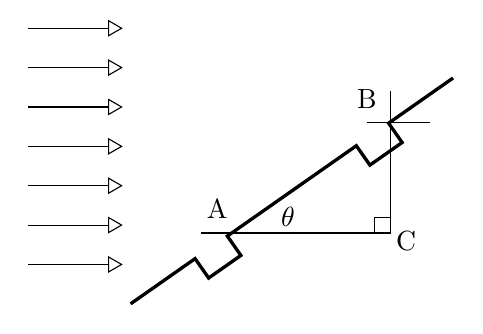
\begin{tikzpicture}
\draw[very thick,shift={(1.5,0)},rotate=35](0,0)--(1,0)--(1,-.3)--(1.5,-.3)--(1.5,0)--(3.5,0)--(3.5,-.3)--(4,-.3)--(4,0)--(5,0);
\foreach \y in {0,.5,...,3}{
\draw[->,-open triangle 60](.2,.5+\y)--(1.4,.5+\y);
}
\draw[](2.4,.9)--(4.8,.9)--(4.8,2.7);
\draw[](4.5,2.3)--(5.3,2.3);
\draw[](4.6,.9)rectangle(4.8,1.1);
%labels
\node[]at(3.5,1.1){$\theta$};
\node[]at(2.6,1.2){A};
\node[]at(4.5,2.6){B};
\node[]at(5,.8){C};
\end{tikzpicture}
\caption{A schematic representation of the grazing incidence technique.}
\label{fig:xr9}
\end{marginfigure}

\item A comparison of the K-shell characteristic x-rays of copper with the accepted values.

\item Discuss whether your results support or refute the hypothesis that x-rays are electromagnetic waves produced in the copper target of the x-ray tube by bremsstrahlung and K-shell interactions and diffracted by the LiF crystal.

\item Using your results, explain why the third and fourth (if visible) peaks are more more likely to be n=2 versions of the first two peaks rather than separate characteristic x-rays.

\item The method of tilting a grating at an extreme angle to effectively get a very small spacing between lines is called the {\bf grazing incidence technique}. Figure \ref{fig:xr9} shows a tilted grating with distance AB between adjacent grooves. Calculate the angle $\theta$ required so that the effective grating spacing BC is 1/1000th the spacing of AB.

\end{enumerate}


\AtEndDocument{\clearpage\ifodd\value{page}\else\null\clearpage\fi} % forces even page count, for double siding

\end{document}
